\section{球径による影響}

球径による影響をより考慮するため,先行研究より拡張した領域に関して考えるため,落下球の直径と終端速度の関係をFig.\ref{fig:diaUT}(a)に示す.落下球の直径が大きくなると,終端速度が指数関数的に高速化した.また,直径と超音波照射による高速化度合の関係をFig.\ref{fig:diaUT}(b)に示す.落下球の直径10[mm]をピークとして超音波照射による高速化が見られた.これらより,式(\ref{eq:Udiff})を用いて整理した結果を,Fig.\ref{fig:muUdiff}に示す.

\begin{figure}[ht]
    \centering
    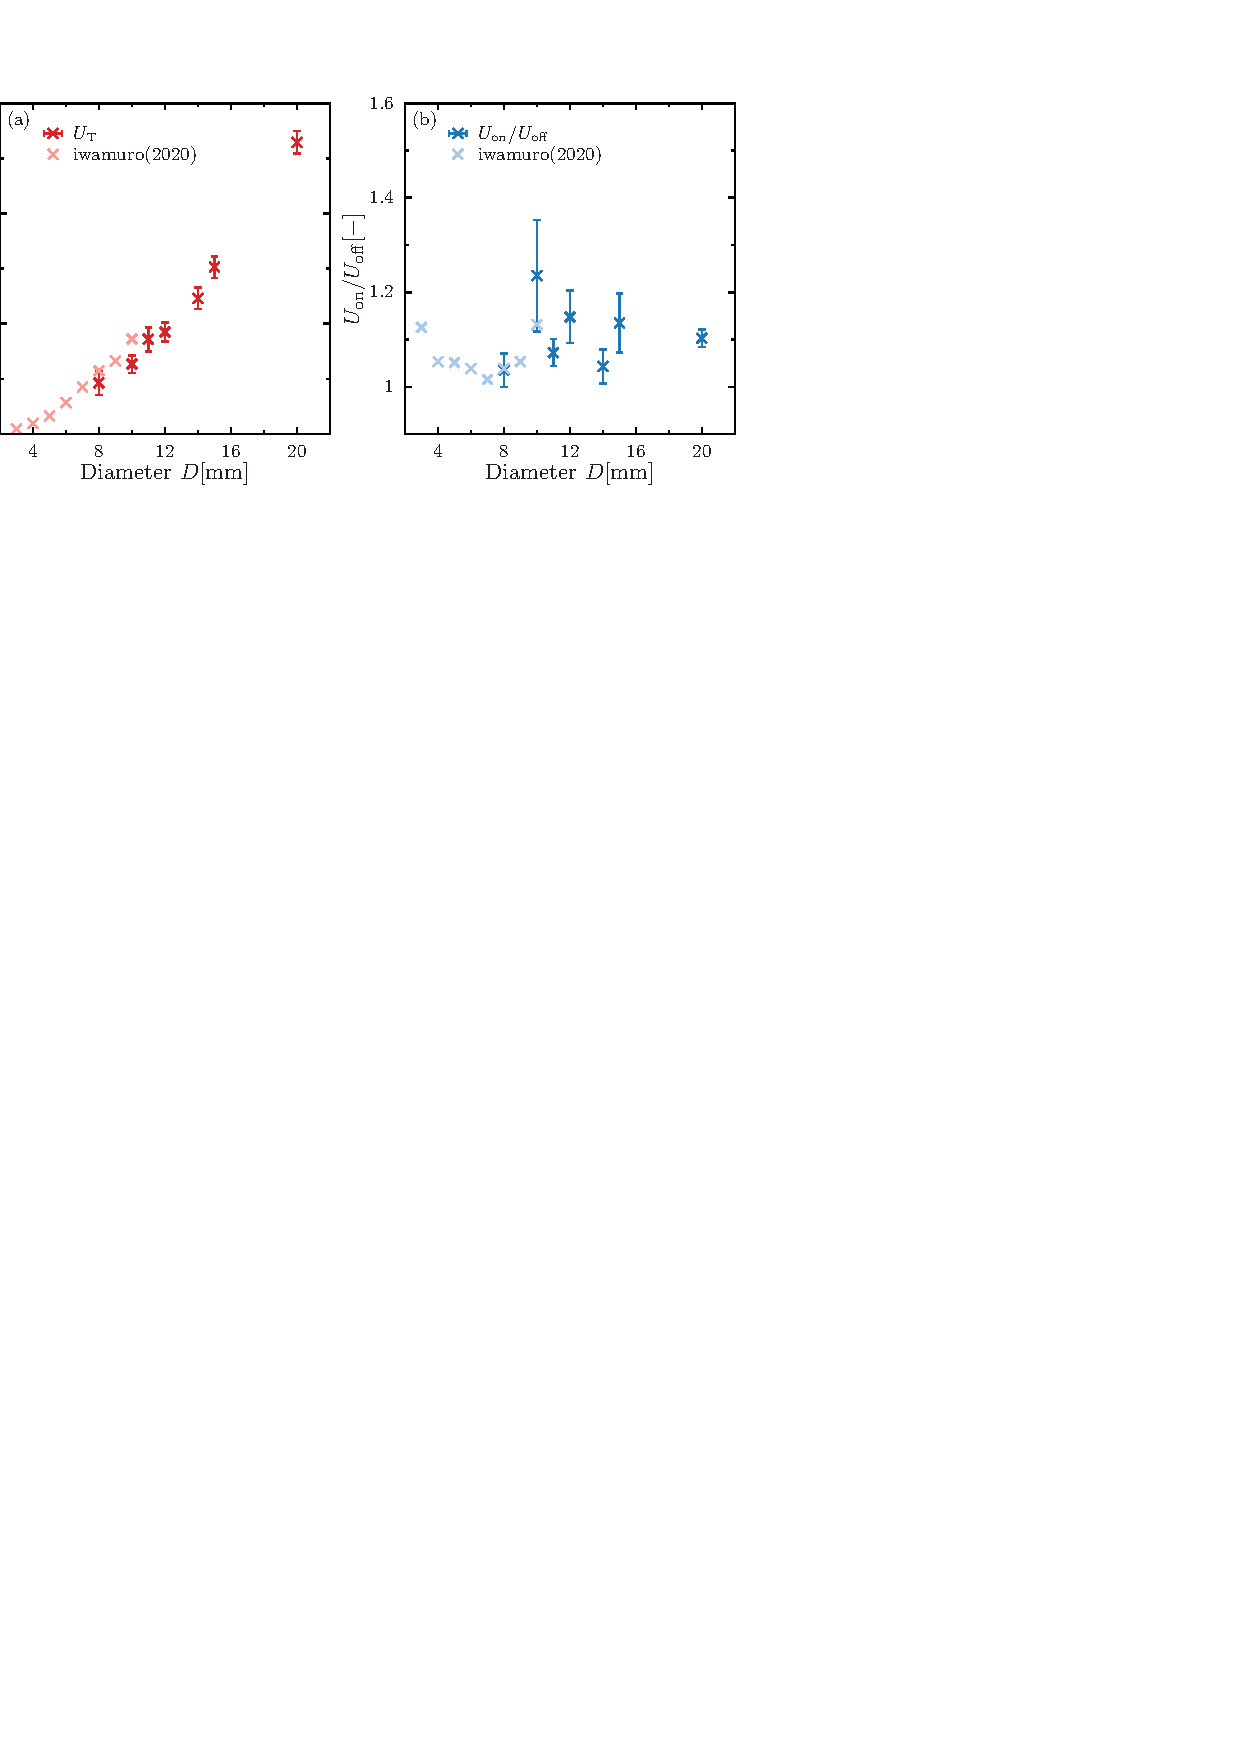
\includegraphics[width=14cm,clip]{./5-Results/diameter/diaUT_Udiff.png}
    \caption{Relationship between diameter and (a)terminal velocity, (b)velocity rato.}
    \label{fig:diaUT}
\end{figure}

\begin{figure}[ht]
    \centering
    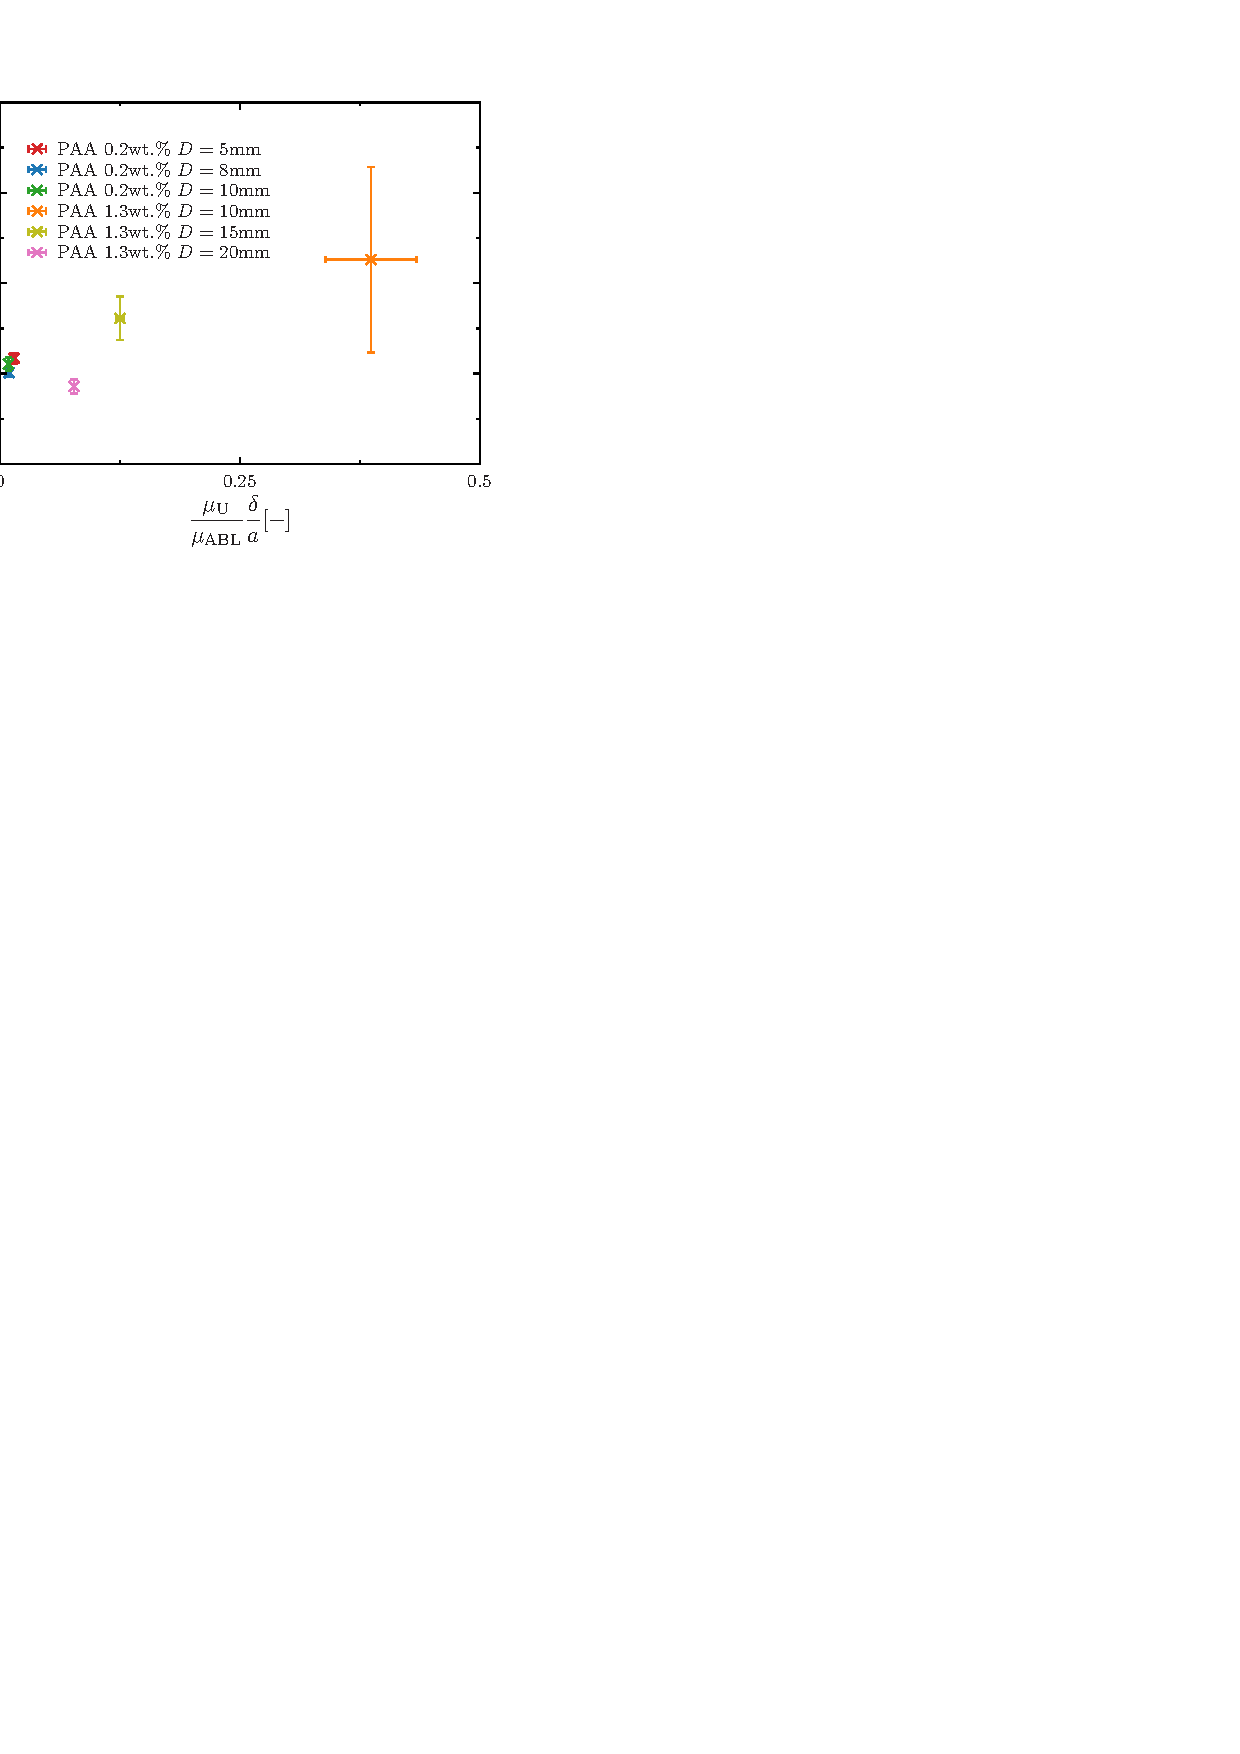
\includegraphics[width=14cm,clip]{./5-Results/diameter/mu_Udiff.png}
    \caption{Relationship between velocity rato and viscosity ratio, the acoustic boundary layer thickness, radius (a)with Iwamuro(2020), (b)without Iwamuro(2020).}
    \label{fig:muUdiff}
\end{figure}